% AMP October 10 methodology checkpoint.
% Independent from the September checkpoint and the comprehensive manuscript.
\documentclass[pdflatex,sn-mathphys-num]{sn-jnl}

\usepackage{graphicx}
\usepackage{booktabs}
\usepackage{longtable}
\usepackage{array}
\usepackage{xcolor}
\usepackage{tikz}
\usetikzlibrary{arrows.meta,fit,positioning}
\newcolumntype{P}[1]{>{\raggedright\arraybackslash}p{#1}}

\begin{document}

\title[AMP-LDP Methodology Checkpoint]
{Weakly Supervised Latent Distribution Profiling for Customer-Level Electricity Theft Detection\\
\large Methodology Checkpoint --- 10 October 2026}

\author*[1]{\fnm{Raghav} \sur{Singh}}
\email{raghav1.mitmpl2024@learner.manipal.edu}

\author[1]{\fnm{Aditya} \sur{Poddar}}
\email{aditya17.mitmpl2024@learner.manipal.edu}

\author[1]{\fnm{Dwijesh} \sur{P}}
\email{dwijesh.mitmpl2024@learner.manipal.edu}

\affil*[1]{\orgdiv{School of Computer Science and Engineering},
  \orgname{Manipal Institute of Technology},
  \orgaddress{\city{Manipal}, \state{Karnataka}, \country{India}}}

\maketitle

\section{Problem Statement}\label{sec:problem}
Electricity theft is a persistent source of non-technical loss in electric-power systems. Beyond lost revenue, irregular and unbilled consumption complicates demand estimation, network planning, and the allocation of field-inspection resources. Smart meters make long consumption histories available at customer level, creating an opportunity to rank customers for investigation using data-driven models rather than relying only on manual rules. Reviews of non-technical-loss detection describe a broad progression from expert rules and engineered indicators to supervised machine learning and deep temporal models \cite{Messinis2018NTLReview}. Established supervised work also shows that consumption histories and customer-profile features contain useful discrimination signal \cite{Buzau2019NTL,Zheng2018WideDeep,Hasan2019CNNLSTM}.

The label available in the State Grid Corporation of China (SGCC) data used by AMP is nevertheless coarser than the measurements. Each customer has a binary \texttt{FLAG}, whereas the consumption record spans many days. The flag identifies a theft-associated customer; it does not identify the day on which theft occurred, its duration, or the particular 30-day window in which a verified event took place. Consequently, copying the customer flag onto every window would create propagated weak labels rather than verified window-level theft annotations. Multiple-instance learning formalizes this distinction: a labelled bag can contain instances whose individual labels are unknown \cite{Carbonneau2018MILSurvey}. For AMP, the customer is the labelled bag and temporal windows are unlabeled instances.

This distinction matters because an unusual consumption segment is not automatically theft-associated. Low usage, missingness, seasonality, occupancy changes, equipment changes, and legitimate behavioural variation can all increase reconstruction error. In the frozen AMP evidence, fully connected, convolutional, and recurrent reconstruction models learned consumption regularities but yielded weak customer-level discrimination when anomaly scores were aggregated. A later supervised diagnostic showed that some discriminative signal existed, yet scoring individually propagated windows still underused the customer label. These findings do not invalidate representation learning; they show that reconstruction abnormality and customer-level theft discrimination are different objectives.

Customer histories are also heterogeneous. Reducing all windows to one mean, one maximum, or one attention-weighted vector can erase information about within-customer variability, tails, and occasional extremes. A customer may be better characterized by the distribution of behaviours across windows than by one representative window or one pooled centroid. Deep time-series research provides many ways to encode local temporal segments \cite{Fawaz2019TimeSeriesReview}, but a suitable customer formulation must preserve useful variation without asserting that any specific window is a theft event.

The practical problem is therefore customer-level ranking under weak temporal supervision and class imbalance. The desired model must use long smart-meter histories, respect the fact that only customers are labelled, retain more than a single summary of their window behaviour, and be assessed with metrics suitable for a rare positive class. Precision--recall analysis is particularly important in imbalanced settings \cite{Saito2015PR}, while imbalance remedies and evaluation choices must be distinguished from the representation itself \cite{He2009Imbalanced}. What remains missing is a governed customer-level formulation that uses window-level temporal structure without pretending that window labels exist, preserves heterogeneity across windows, and isolates the value of learned representations from the value of aggregation itself.


\section{Literature Survey}\label{sec:literature-survey}

The literature on data-driven electricity-theft detection spans engineered customer profiles, supervised temporal classifiers, reconstruction and representation learning, graph and transfer models, clustering, and class-imbalance strategies. The studies reviewed here are the 24 journal articles admitted by the Stage 29 verification protocol. Fifteen were published during 2023--2026. Their titles, authors, journals, years, and DOIs were checked against publisher and Crossref records, and journal indexing was substantiated at journal level. The survey therefore emphasizes verified design information and avoids converting heterogeneous reported scores into a leaderboard.

Three distinctions guide the synthesis. First, a customer-level label is not a timestamped event label. Second, using the same dataset name does not guarantee the same customers, preprocessing, prevalence, split, balancing, tuning, or evaluation unit. Third, ROC-AUC, Average Precision, accuracy, and threshold-dependent measures answer different questions, especially under class imbalance. Reported values below remain attached to their source protocols and are not treated as directly comparable with AMP-LDP.

\subsection{Conventional supervision and engineered customer profiles}

Earlier non-technical-loss research established the customer as a useful prediction unit. Messinis and Hatziargyriou reviewed detection families, data sources, and evaluation issues, showing that non-technical-loss studies differ substantially in assumptions and protocol \cite{Messinis2018NTLReview}. Buzau et al. used utility smart-meter data and inspected non-technical-loss targets with supervised learning and engineered features, demonstrating the practical strength of customer-profile models \cite{Buzau2019NTL}. Shehzad et al. combined big-data processing and genetic-algorithm optimization for supervised electricity-theft classification on SGCC histories \cite{Shehzad2022GeneticETD}. These approaches motivate the FULL\_48 comparator in AMP: a strong engineered customer profile should not be displaced by a learned method unless the comparison is governed and informative.

\subsection{Deep temporal representation learning}

Deep models increasingly transform a long customer history before classification. Zheng et al. combined wide and deep convolutional views of SGCC consumption, including one- and two-dimensional temporal representations \cite{Zheng2018WideDeep}. Hasan et al. combined convolutional feature extraction with an LSTM and used SMOTE to address imbalance \cite{Hasan2019CNNLSTM}. More broadly, the time-series classification review by Ismail Fawaz et al. documents convolutional, recurrent, and hybrid mechanisms for learning temporal representations \cite{Fawaz2019TimeSeriesReview}. This body of work supports learning from temporal structure, but it does not by itself resolve the label-granularity question: a representation can be learned from a full history while the location of the event remains unknown.

\subsection{Reconstruction, weak supervision, and aggregation}

Autoencoders are often used either to reduce dimensionality or to score deviations from reconstructed normal behaviour. In the verified recent set, Pamir et al. use a gated convolutional autoencoder as a feature extractor inside a supervised, cost-sensitive LSTM pipeline rather than treating reconstruction error alone as the final theft decision \cite{Pamir2023EnergyOptimization}. That distinction is important. Reconstruction objectives reward faithful reproduction of common structure; they do not necessarily align with the ranking of theft-associated customers. AMP's own frozen reconstruction experiments reached the same methodological conclusion and motivated a customer-supervised formulation.

Multiple-instance learning provides a principled vocabulary for customer bags and unlabeled windows \cite{Carbonneau2018MILSurvey}. However, an MIL architecture still needs an aggregation rule. Mean, maximum, and attention pooling each produce a single vector and can discard distributional structure. AMP therefore treats weak supervision and aggregation as separate design questions: the loss remains customer-level, while the representation retains several statistics of the customer's latent-window distribution.

\subsection{Class imbalance and evaluation}

The theft class is a minority in SGCC and many operational datasets. He and Garcia review data-level, algorithm-level, and hybrid responses to imbalanced learning \cite{He2009Imbalanced}. Recent theft studies use class weighting, undersampling, SMOTE variants, or generative procedures, but those choices can change the effective training distribution and complicate comparison. Saito and Rehmsmeier show that precision--recall plots are more informative than ROC plots alone when positives are rare \cite{Saito2015PR}. AMP therefore treats ROC-AUC and Average Precision as co-primary customer-level metrics and avoids accuracy as a primary measure.

\subsection{Recent paper-wise analysis: 2023--2026}

\paragraph{Liu et al. (2023).}
Liu et al. sought to improve electricity-theft detection by learning differences among customer representations rather than relying only on independently encoded histories \cite{Liu2023ContrastiveETD}. On SGCC customer histories with customer-level normal/theft targets, they combined a supervised contrastive encoder, largest-triangle-three-buckets augmentation, and a classification objective. The paper evaluates AUC and recall and reports favourable results under its SGCC protocol. Its relevance is the explicit use of learned customer representations. The verified evidence does not establish a matched direct-distribution control, and its customer partition is not the governed AMP split; its scores are therefore contextual rather than directly comparable.

\paragraph{Pamir et al. (2023).}
Pamir et al. addressed dimensionality and class imbalance in SGCC electricity-theft classification \cite{Pamir2023EnergyOptimization}. Their pipeline combines cost-sensitive learning, a gated convolutional autoencoder, an LSTM classifier, and salp-swarm hyperparameter tuning. The article states 42,372 customer histories, 3,615 theft customers, and an 80/20 train/test split. It reports 99.45\% precision, 95.93\% F1, 92.25\% accuracy, and 71.13\% AUC. The unusual divergence among these metrics reinforces the need to preserve source definitions and prevalence. Extensive tuning and the absence of AMP's frozen cohorts prevent protocol-level comparison.

\paragraph{Khan et al. (2023).}
Khan et al. investigated an AlexNet-derived deep classifier for customer-level electricity-theft detection on CNGC/SGCC consumption histories \cite{Khan2023AlexNet}. The verified package records imbalance treatment and evaluation with accuracy, precision, recall, F1, and AUC. The study supports the conclusion that deep full-history models can extract discriminative consumption patterns. Exact protocol equivalence with AMP was not established: its sampling, model tuning, and split differ, and no matched direct-versus-latent distribution comparison is reported. Accordingly, the paper informs the temporal-classifier context rather than a numerical ranking.

\paragraph{Huang et al. (2024).}
Huang et al. proposed dual-time feature fusion to combine complementary temporal views of SGCC daily customer histories \cite{Huang2024DualTime}. Under the paper's customer-supervised split, the reported values are 0.947 accuracy, 0.932 precision, 0.964 recall, 0.948 F1, and 0.986 AUC. The findings show that multi-scale temporal organization can be useful for theft-associated customer classification. Average Precision was not reported in the verified comparison record, and the preprocessing and split are not AMP-governed. The model also studies temporal fusion rather than the specific question of preserving the distribution of unlabeled windows.

\paragraph{Zhuang et al. (2024).}
Zhuang et al. developed a dynamic generative residual graph convolutional network for electricity-theft detection on SGCC customer histories \cite{Zhuang2024GraphETD}. The objective is to exploit relational or graph-structured dependencies while augmenting the representation through a generative component. The article reports classification metrics under its own preprocessing and partition. The approach broadens the temporal deep-learning family beyond sequence-only models, but a precise point finding suitable for transcription was not established by the Stage 29 package. For AMP's question, graph construction and generative augmentation change several factors simultaneously; the verified evidence does not isolate aggregation or provide a matched direct-feature control.

\paragraph{Shahzadi et al. (2024).}
Shahzadi et al. proposed a data-driven artificial-intelligence pipeline for energy-theft detection in urbanized smart grids using SGCC customer histories \cite{Shahzadi2024Urbanized}. The verified record identifies a deep-learning approach with imbalance handling and reports the standard accuracy, precision, recall, F1, and AUC family under a paper-specific partition. The study is relevant as a recent supervised SGCC benchmark. The verified package establishes the metric family but not an exact point finding suitable for transcription, so no value is reproduced here. Optimization, preprocessing, and evaluation differences limit direct comparison with AMP-LDP.

\paragraph{Tursunboev et al. (2024).}
Tursunboev et al. combined multi-objective evolutionary optimization with hybrid deep learning for energy-theft detection on SGCC customer histories \cite{Tursunboev2024MultiObjective}. The objective is to improve supervised customer classification by optimizing competing model goals. The article reports customer-level classification metrics within its internally optimized protocol. It illustrates the performance-oriented search direction in recent electricity-theft research, while the Stage 29 package does not establish an exact point finding for transcription. The search budget, optimization objectives, and lack of a separately frozen external cohort differ from AMP's governance; the verified package therefore supports only a structural comparison, not a transfer of headline scores.

\paragraph{Wang et al. (2024).}
Wang et al. studied a two-stage approach intended to generalize electricity-theft detection to new regions \cite{Wang2024NewRegions}. The environment contains source and new-region theft data, and the evaluation focuses on performance under regional transfer. The verified finding is protocol-level evidence from a cross-region assessment; an exact point result was not established for this package. This is important because it targets a limitation that AMP does not resolve: evidence from one source does not establish utility- or region-level generalization. The method and metrics are tied to the paper's cross-region protocol, which differs from AMP's within-SGCC governed cohorts.

\paragraph{Iftikhar et al. (2024).}
Iftikhar et al. addressed high dimensionality and imbalance in CNGC/SGCC customer histories using K-means SMOTE with an MLP--GRU classifier \cite{Iftikhar2024MLPGRU}. They report precision, recall, F1, accuracy, MCC, ROC-AUC, and PR-AUC across 50/50, 75/25, and 90/10 train/test ratios; the Stage 29 record notes a displayed best AUC of 0.95. The multi-ratio analysis demonstrates split sensitivity. Synthetic balancing and the absence of fixed cohort identities make the protocol unlike AMP's natural-prevalence, governed evaluation, so the value is not used as a direct comparator.

\paragraph{Saqib et al. (2024).}
Saqib et al. examined deep-learning-based electricity-theft prediction in a non-smart-grid billing or consumption environment with a customer theft target \cite{Saqib2024NonSmartGrid}. The article evaluates a supervised deep predictor with classification metrics under its own split. Its principal contribution to this review is environmental breadth: theft-detection systems may operate with data and infrastructure different from SGCC smart-meter histories. A precise point finding was not established by Stage 29, and those differences in acquisition setting and feature availability also limit comparability; no numerical result is inferred.

\paragraph{Elshennawy et al. (2025).}
Elshennawy et al. proposed a hybrid deep-learning classifier for electricity-theft detection on SGCC customer histories \cite{Elshennawy2025EfficientETD}. The study uses customer supervision and reports accuracy up to 94.7\%, together with other classification measures, under its article-specific protocol. It provides recent evidence that hybrid deep representations can discriminate SGCC customer labels. The verified record does not establish alignment with AMP's preprocessing, prevalence, split membership, or paired controls. The reported accuracy is therefore retained as a source-specific result rather than evidence of superiority over or inferiority to AMP-LDP.

\paragraph{Iqbal et al. (2025).}
Iqbal et al. investigated transfer learning for temporal electricity sequences using CNN--LSTM and BiGRU--BiLSTM models \cite{Iqbal2025TransferTemporal}. The customer-level evaluation reports precision, recall, F1, accuracy, and ROC-AUC, with ROC-AUC up to 0.89 in the article protocol. The work shows how temporal representations can be transferred rather than trained only within one target sample. The construction of source and target data differs from AMP's fixed DEV\_TRAIN, DEV\_VAL, CONFIRMATION, and final roles; the result therefore provides methodological context but not a protocol-equivalent benchmark.

\paragraph{Yang et al. (2026).}
Yang et al. combined a temporal convolutional network with Bayesian hyperparameter optimization and post-hoc explainability for electricity-theft classification \cite{Liupeng2026ExplainableETD}. The paper uses customer consumption time series and reports 98.04\% accuracy under its own stratified protocol. Its objective spans temporal feature learning, parameter search, and explanation through feature-attribution methods. Accuracy is sensitive to prevalence, and the cohort and tuning procedure are not AMP-equivalent. The paper is relevant to temporal convolution and interpretability, but its result cannot be inserted into an AMP leaderboard.

\paragraph{Yang et al. (2024).}
Zhengqiang Yang et al. proposed a self-decision ant-colony clustering algorithm for electricity-theft detection and assessed it on SGCC and Smart* household data \cite{Yang2024AntColony}. The method is an unsupervised clustering approach followed by evaluation against customer or household labels, offering a non-neural alternative to supervised deep models. The verified finding is that the method received dataset-specific classification assessment; the package does not establish a single point estimate suitable for AMP comparison. Use of two datasets and a clustering objective changes the scientific question relative to calibrated customer-probability modelling.

\paragraph{Gunduz and Das (2024).}
Gunduz and Das investigated a hybrid CNN-based security approach for detecting energy theft from consumption patterns \cite{Gunduz2024HybridCNN}. The verified record identifies constructed or injected attack patterns, generative data treatment, and evaluation through accuracy, precision, recall, F1, and ROC analysis. The study demonstrates a controlled attack-pattern setting in which convolutional models can be tested, although the verified package does not establish an exact point finding for transcription. Its labels are not equivalent to SGCC's inspected customer flag: synthetic or constructed attacks provide temporal and behavioural assumptions absent from the AMP data. This protocol difference is the central limitation for comparison.

\subsection{Comparative view of recent journal studies}

Table~\ref{tab:recent-literature} consolidates the 15 verified journal papers from 2023--2026. Metrics are reported only at the level substantiated by the Stage 29 package. A metric name without a value means that the paper evaluated the measure but the verified package did not establish a point estimate suitable for transcription.

\begingroup
\small
\setlength{\tabcolsep}{3pt}
\begin{longtable}{@{}P{0.13\textwidth}P{0.18\textwidth}P{0.16\textwidth}P{0.25\textwidth}P{0.20\textwidth}@{}}
\caption{Recent electricity-theft journal literature. Values are source-protocol results and are not a cross-paper leaderboard.}\label{tab:recent-literature}\\
\toprule
Author and year & Technique & Dataset & Performance metrics & Limitation \\
\midrule
\endfirsthead
\toprule
Author and year & Technique & Dataset & Performance metrics & Limitation \\
\midrule
\endhead
\midrule
\multicolumn{5}{r}{Continued on next page}\\
\endfoot
\bottomrule
\endlastfoot
Liu et al. (2023) & Supervised contrastive encoder with LTTB augmentation & SGCC customer histories & AUC and recall under paper split & No matched direct-distribution control; non-AMP split \\
Pamir et al. (2023) & Cost-sensitive GCAE--LSTM with salp-swarm tuning & SGCC; 42,372 histories, 3,615 theft customers & Precision 99.45\%; F1 95.93\%; accuracy 92.25\%; AUC 71.13\%; 80/20 split & Extensive tuning; metric divergence; protocol not equivalent \\
Khan et al. (2023) & AlexNet-derived classifier with imbalance treatment & CNGC/SGCC customer histories & Accuracy, precision, recall, F1, AUC & Sampling and tuning differ; no matched aggregation control \\
Huang et al. (2024) & Dual-time feature fusion & SGCC daily histories & Accuracy 0.947; precision 0.932; recall 0.964; F1 0.948; AUC 0.986 & No AP in verified record; non-governed split \\
Zhuang et al. (2024) & Dynamic generative residual GCN & SGCC customer histories & Classification metrics under paper protocol & Graph and generative components confound representation comparison \\
Shahzadi et al. (2024) & Deep data-driven pipeline with imbalance handling & SGCC customer histories & Accuracy, precision, recall, F1, AUC & Exact verified point values unavailable; different partition \\
Tursunboev et al. (2024) & Multi-objective evolutionary hybrid deep learning & SGCC customer histories & Customer classification metrics & Search budget and objectives differ; no frozen external cohort \\
Wang et al. (2024) & Two-stage regional-transfer detector & Source and new-region theft data & Cross-region classification assessment & Different target and datasets; not an AMP cohort comparison \\
Iftikhar et al. (2024) & K-means SMOTE with MLP--GRU & CNGC/SGCC customer histories & Precision, recall, F1, accuracy, MCC, ROC-AUC, PR-AUC; displayed best AUC 0.95 across three split ratios & Synthetic balancing and changing train/test ratios \\
Saqib et al. (2024) & Deep supervised predictor & Non-smart-grid billing/consumption setting & Classification metrics under paper split & Different acquisition environment and feature availability \\
Elshennawy et al. (2025) & Hybrid deep classifier & SGCC customer histories & Accuracy up to 94.7\%; other classification metrics & Preprocessing, prevalence, and partition not AMP-equivalent \\
Iqbal et al. (2025) & Transfer-learned CNN--LSTM and BiGRU--BiLSTM & Temporal electricity sequences & Precision, recall, F1, accuracy, ROC-AUC; AUC up to 0.89 & Source/target construction differs from governed AMP roles \\
Yang et al. (2026) & Bayesian-optimized TCN with explainability & Customer consumption sequences & Accuracy 98.04\% under article protocol & Accuracy prevalence-sensitive; tuning and cohort differ \\
Yang et al. (2024) & Self-decision ant-colony clustering & SGCC and Smart* & Dataset-specific classification metrics & Unsupervised objective and two datasets differ from probability modelling \\
Gunduz and Das (2024) & Hybrid CNN with generative treatment & Constructed or injected consumption attacks & Accuracy, precision, recall, F1, ROC & Synthetic attacks are not inspected SGCC customer labels \\
\end{longtable}
\endgroup

\subsection{Synthesis and methodological boundary}

Across the recent papers, the dominant formulation is supervised classification of a complete customer history or a transformed version of that history. Contrastive, convolutional, recurrent, graph, transfer, clustering, evolutionary, and explainable-AI approaches expand the representation toolkit \cite{Liu2023ContrastiveETD,Khan2023AlexNet,Huang2024DualTime,Zhuang2024GraphETD,Tursunboev2024MultiObjective,Wang2024NewRegions,Iqbal2025TransferTemporal,Liupeng2026ExplainableETD,Yang2024AntColony}. Imbalance is addressed through weighting, undersampling, SMOTE variants, and generative procedures \cite{Pamir2023EnergyOptimization,Iftikhar2024MLPGRU,Gunduz2024HybridCNN}. What varies just as strongly is the experimental protocol.

The literature therefore supports several robust qualitative conclusions: smart-meter histories contain customer-level signal; learned temporal representations can be useful; imbalance must be handled and evaluated explicitly; and external-region testing is a distinct objective. It does not support a common numerical ranking. SGCC studies may use different customer subsets, missing-value rules, synthetic balancing, split ratios, model-selection procedures, and evaluation units. Non-smart-grid and constructed-attack studies differ even more fundamentally \cite{Saqib2024NonSmartGrid,Gunduz2024HybridCNN}.

For AMP, the central unresolved issue is not the availability of another deep architecture. It is the combination of label granularity and aggregation. The verified set does not establish a study that jointly treats windows as unlabeled instances under a customer label, learns window representations without an instance theft loss, preserves their within-customer distribution, compares that distribution with identical direct-feature statistics, and freezes the resulting comparison across separate governed cohorts. This statement is bounded to the verified 24-paper set and is not a universal novelty claim.


\section{Research Gap and Study Objectives}\label{sec:gap-objectives}

\subsection{Bounded research gap}

The reviewed literature establishes a rich set of customer-supervised classifiers but exposes recurring limitations. Full-history CNN, recurrent, graph, and contrastive models learn useful representations, yet most papers do not isolate whether an improvement comes from the encoder, the aggregation rule, the classifier, balancing, or hyperparameter search. Autoencoder components are commonly embedded in supervised pipelines, while reconstruction error by itself is not guaranteed to align with customer theft discrimination. Class-balancing strategies alter the effective training distribution, and heterogeneous SGCC partitions prevent direct comparison of headline metrics.

More fundamentally, the measurement and label granularities differ. SGCC supplies one customer \texttt{FLAG}, not verified theft-event timing. A 30-day window is therefore an unlabeled instance. Treating every window from a flagged customer as positive assumes that theft spans the whole history and turns a bag label into pseudo instance labels. Conversely, collapsing all windows into a single mean, maximum, or attention vector can remove variability, tails, and extremes that distinguish customer behaviour. Weak supervision defines the first problem; distribution-preserving aggregation addresses the second.

The matched-control requirement follows from this distinction. If a latent distribution model is compared only with single-vector MIL, any gain may reflect the richer six-statistic aggregation rather than learned encoding. AMP therefore compares two representations under the same statistics and HGB classifier: DIRECT aggregates the 17 handcrafted window summaries, while AMP-LDP aggregates 16 learned latent dimensions. FULL\_48 supplies a separate strong engineered profile. This design permits the narrower question, ``Does learned encoding add value once aggregation is held constant?''

Evaluation governance is equally important. Development evidence can motivate a hypothesis but can also be optimistic. AMP consequently separates DEV\_VAL, CONFIRMATION, and terminal final-evaluation roles; freezes model, seed, ensemble, comparator, metric, and bootstrap policies before opening later cohorts; and uses paired customer comparisons. This evidence chain does not make the final cohort pristine: it had disclosed historical access for an obsolete baseline. It does make the current Study 2 comparison auditable and prevents post-result rescue experiments.

Within the 24 verified journal articles, no paper was found that simultaneously combines customer-only labels, unlabeled temporal windows, learned window representations, matched direct-versus-latent distribution aggregation, and frozen replication across three governed cohort roles. This is a bounded observation about the verified set, not a claim that AMP-LDP is the first such method in all published literature.

\subsection{Primary research question}

\begin{quote}
Under customer-level SGCC theft labels and no verified theft-event timestamps, does learning representations of unlabeled consumption windows before distribution-preserving customer aggregation improve customer-level discrimination beyond applying the same aggregation directly to handcrafted window features?
\end{quote}

\subsection{Study objectives}

The completed study pursued the following measurable objectives:

\begin{enumerate}
  \item \textbf{Respect the available supervision.} Formulate each customer as a bag of 30-day windows, apply theft supervision only at customer level, and avoid claims about individual theft windows or event timing.
  \item \textbf{Test the aggregation bottleneck.} Evaluate whether single-vector mean, maximum, and gated-attention MIL retain sufficient customer information, and compare their customer-level ROC-AUC and Average Precision with multi-statistic distribution representations.
  \item \textbf{Isolate learned-representation value.} Hold the six distribution statistics and HGB classifier constant while comparing AMP-LDP's 96-dimensional latent distribution with the 102-dimensional DIRECT distribution of handcrafted window summaries.
  \item \textbf{Benchmark against an established customer profile.} Compare the frozen AMP-LDP ensemble with the DEV\_TRAIN-fitted FULL\_48 HGB comparator under symmetric Study 2 training governance.
  \item \textbf{Evaluate reproducibility and uncertainty.} Assess the frozen five-seed arithmetic ensemble on DEV\_VAL, CONFIRMATION, and the governed final evaluation; report individual-seed robustness and paired customer-bootstrap intervals for ROC-AUC and Average Precision differences.
  \item \textbf{Constrain the resulting claims.} Determine whether the learned-distribution effect persists across cohort roles while explicitly withholding claims of theft-period localization, causal identification, external-utility generalization, and protocol-independent state-of-the-art performance.
\end{enumerate}

These objectives describe the completed AMP evidence chain rather than a proposed future experiment. The remaining report sections document the frozen implementation and results; no new model development is implied.


\section{Methodology}\label{sec:methodology}

\subsection{Overall System Architecture}\label{sec:architecture}

AMP---Automated Meter Profiling for Electricity Theft Detection---is implemented as a customer-level machine-learning pipeline. Figure~\ref{fig:amp-architecture} summarizes the data flow. The input is the State Grid Corporation of China (SGCC) customer-by-day table. Preprocessing repairs the calendar, fills missing values within each customer history, applies a logarithmic transform, and scales each daily position using training-customer statistics. Customers are then assigned to disjoint development, confirmation, and final-evaluation roles before temporal examples are generated. Each customer history is divided into eligible 30-day windows, and every window is converted into 17 behavioural summaries.

AMP-LDP maps each 17-dimensional window vector to a 16-dimensional latent vector. Instead of labelling or classifying individual windows, it describes the distribution of every latent dimension across all windows belonging to one customer. Six statistics per latent dimension produce a 96-dimensional customer profile. A HistGradientBoosting (HGB) classifier converts this profile into a customer-level theft-discrimination probability. Five independently seeded encoder--HGB pipelines are combined by arithmetic averaging. The final output is one probability or ranking score per customer; it is not a probability for any particular 30-day period.

\begin{figure*}[t]
  \centering
  % Reproducible TikZ source for the frozen AMP-LDP architecture.
\resizebox{\textwidth}{!}{%
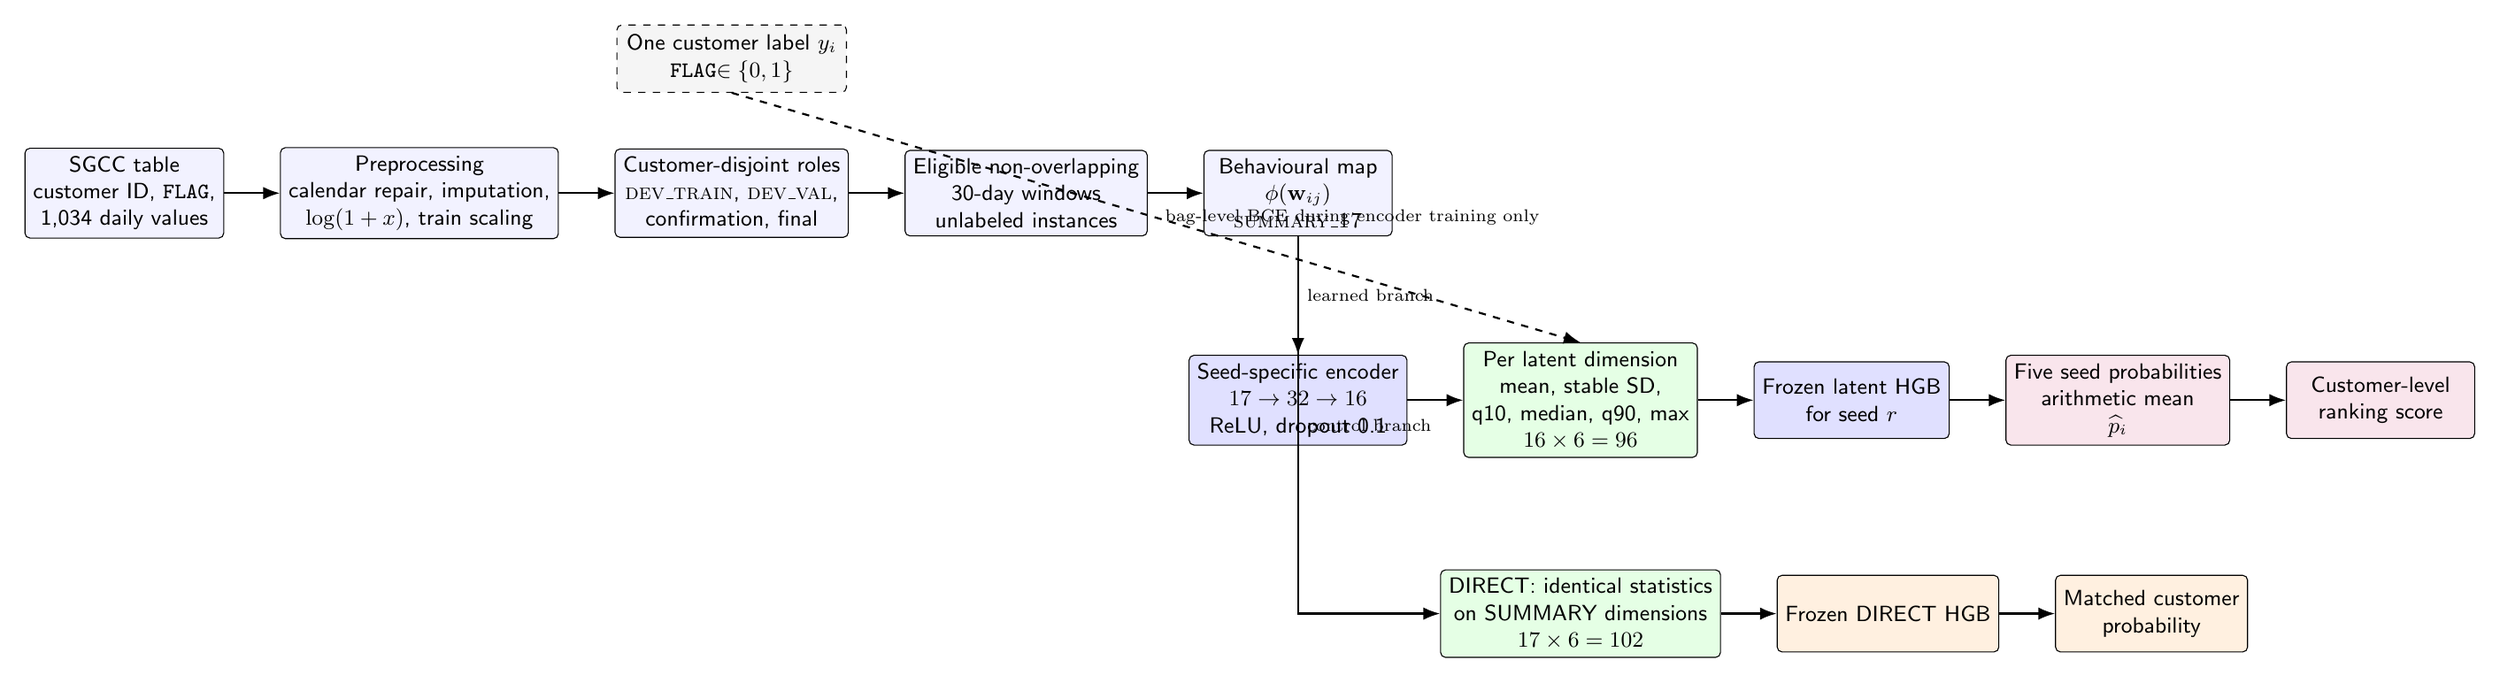
\begin{tikzpicture}[
  font=\sffamily\small,
  node distance=8mm and 8mm,
  block/.style={draw, rounded corners=2pt, align=center, minimum height=11mm, minimum width=27mm, fill=blue!5},
  learned/.style={block, fill=blue!12},
  aggregate/.style={block, fill=green!10},
  control/.style={block, fill=orange!12},
  output/.style={block, fill=purple!10},
  note/.style={draw, dashed, rounded corners=2pt, align=center, fill=gray!8, inner sep=4pt},
  arrow/.style={-{Latex[length=2.4mm]}, thick},
  dashedarrow/.style={-{Latex[length=2.4mm]}, thick, dashed}
]
  \node[block] (sgcc) {SGCC table\\customer ID, \texttt{FLAG},\\1,034 daily values};
  \node[block, right=of sgcc] (prep) {Preprocessing\\calendar repair, imputation,\\$\log(1+x)$, train scaling};
  \node[block, right=of prep] (split) {Customer-disjoint roles\\\textsc{dev\_train}, \textsc{dev\_val},\\confirmation, final};
  \node[block, right=of split] (windows) {Eligible non-overlapping\\30-day windows\\unlabeled instances};
  \node[block, right=of windows] (summary) {Behavioural map\\$\phi(\mathbf w_{ij})$\\\textsc{summary\_17}};

  \node[note, above=of split] (flag) {One customer label $y_i$\\\texttt{FLAG}$\in\{0,1\}$};
  \node[learned, below=17mm of summary] (encoder) {Seed-specific encoder\\$17\rightarrow32\rightarrow16$\\ReLU, dropout 0.1};
  \node[aggregate, right=of encoder] (latentpool) {Per latent dimension\\mean, stable SD,\\q10, median, q90, max\\$16\times6=96$};
  \node[learned, right=of latentpool] (hgb) {Frozen latent HGB\\for seed $r$};
  \node[output, right=of hgb] (ensemble) {Five seed probabilities\\arithmetic mean\\$\widehat p_i$};
  \node[output, right=of ensemble] (decision) {Customer-level\\ranking score};

  \node[aggregate, below=16mm of latentpool] (directpool) {DIRECT: identical statistics\\on SUMMARY dimensions\\$17\times6=102$};
  \node[control, right=of directpool] (directhgb) {Frozen DIRECT HGB};
  \node[control, right=of directhgb] (directprob) {Matched customer\\probability};

  \draw[arrow] (sgcc) -- (prep);
  \draw[arrow] (prep) -- (split);
  \draw[arrow] (split) -- (windows);
  \draw[arrow] (windows) -- (summary);
  \draw[arrow] (summary) -- node[right, font=\scriptsize]{learned branch} (encoder);
  \draw[arrow] (encoder) -- (latentpool);
  \draw[arrow] (latentpool) -- (hgb);
  \draw[arrow] (hgb) -- (ensemble);
  \draw[arrow] (ensemble) -- (decision);
  \draw[arrow] (summary.south) |- node[pos=0.25, right, font=\scriptsize]{control branch} (directpool.west);
  \draw[arrow] (directpool) -- (directhgb);
  \draw[arrow] (directhgb) -- (directprob);
  \draw[dashedarrow] (flag.south) -- node[right, font=\scriptsize]{bag-level BCE during encoder training only} (latentpool.north);

\end{tikzpicture}%
}

  \caption{Implemented AMP-LDP pipeline and matched DIRECT control. The customer label supervises encoder training once per customer bag and is never attached to individual windows.}
  \label{fig:amp-architecture}
\end{figure*}

\subsection{Dataset Description}\label{sec:dataset}

The project uses the publicly distributed SGCC smart-meter benchmark, which has also been used in earlier customer-level electricity-theft studies \cite{Zheng2018WideDeep,Shehzad2022GeneticETD}. Each row contains a customer identifier, a binary \texttt{FLAG}, and chronological daily electricity-consumption measurements. The repository does not independently establish the utility's inspection procedure or theft-event dates, so those details are not inferred.

Cleaning retained 42,367 customers: 38,755 labelled normal and 3,612 theft-associated, giving a theft prevalence of 8.5255\%. Five source rows containing no observed consumption values were removed. Calendar validation produced 1,034 daily positions. The almost entirely missing date 3 October 2014 was removed, while the absent date 18 September 2016 was inserted as an explicitly missing position so that calendar order remained correct.

Missing values were handled separately within each customer series. Internal gaps were linearly interpolated; leading and trailing gaps were filled using the nearest observed value. Zero consumption remained a valid reading. The numerical sequence was transformed using $\log(1+x)$ without manual clipping, and a separate binary mask preserved whether each value had originally been observed. A feature-wise standard scaler was fitted only on historical-training customers and applied unchanged to the other customer partitions. The mask, customer identifier, label, split name, and missing-value counts were excluded from model inputs.

The original customers were split once by customer, not by window, using a deterministic 70/15/15 stratified split with seed 42. The original training group was later divided 80/20 into \textsc{dev\_train} and \textsc{dev\_val}; the original validation group became \textsc{confirmation}; and the original test group became the final evaluation cohort. Table~\ref{tab:cohorts} records the frozen customer counts. One theft-labelled \textsc{dev\_train} customer had no eligible 30-day window. It remained in the governance manifest but was excluded from representation fitting, leaving 23,724 representation-available training customers. All pairwise customer overlaps between roles are zero.

\begin{table}[ht]
\centering
\caption{Frozen customer-level research roles.}
\label{tab:cohorts}
\small
\begin{tabular}{@{}lrrrr@{}}
\toprule
Role & Customers & Normal & Theft & Prevalence \\
\midrule
\textsc{dev\_train} & 23,725 & 21,702 & 2,023 & 8.5269\% \\
\textsc{dev\_val} & 5,931 & 5,426 & 505 & 8.5146\% \\
\textsc{confirmation} & 6,355 & 5,813 & 542 & 8.5287\% \\
Final evaluation & 6,356 & 5,814 & 542 & 8.5274\% \\
\bottomrule
\end{tabular}
\end{table}

Each scaled history was divided into complete, non-overlapping windows of 30 days, using window length 30 and stride 30. The 1,034 daily positions permit at most 34 complete windows; the final 14 positions do not form a complete window and were unused. A window was eligible when at least one of its 30 positions had originally been observed. A fully originally missing window was removed even if interpolation had produced finite values.

For each retained window $\mathbf{w}_{ij}\in\mathbb{R}^{30}$, a fixed map $\phi$ produces $\mathbf{s}_{ij}=\phi(\mathbf{w}_{ij})\in\mathbb{R}^{17}$. The 17 summaries are mean, median, minimum, maximum, 10th and 90th percentiles, population standard deviation, range, interquartile range, mean absolute deviation, signed and absolute first-to-last change, mean and maximum absolute consecutive change, least-squares slope, fraction at or below $-1$ in scaled space, and second-half minus first-half mean. These summary dimensions were standardized using means and population standard deviations calculated from all eligible \textsc{dev\_train} windows only.

The label granularity is important. For customer $i$, let
\begin{equation}
  \mathcal{B}_i=\{\mathbf{s}_{ij}:j=1,\ldots,m_i\},
  \qquad y_i\in\{0,1\}.
  \label{eq:bag}
\end{equation}
The \texttt{FLAG} $y_i$ labels the complete customer bag $\mathcal{B}_i$. It does not identify a theft date, duration, or verified positive window. Copying $y_i$ to every window would therefore create assumed instance labels. AMP-LDP instead uses one customer-level loss and makes no theft-localization claim.

\subsection{Proposed Model and Comparison Approaches}\label{sec:model}

For each seed $r\in\{42,43,44,45,46\}$, the standardized window vector $\widetilde{\mathbf{s}}_{ij}$ is encoded as
\begin{equation}
 \mathbf{z}_{ij}^{(r)}=operatorname{ReLU}\!\left(
 \mathbf{W}_{2}^{(r)}\operatorname{Drop}_{0.1}\!\left[
 \operatorname{ReLU}\!\left(\mathbf{W}_{1}^{(r)}\widetilde{\mathbf{s}}_{ij}
 +\mathbf{b}_{1}^{(r)}\right)\right]+\mathbf{b}_{2}^{(r)}\right)
 \in\mathbb{R}^{16}.
 \label{eq:encoder}
\end{equation}
This is the implemented $17\rightarrow32\rightarrow16$ encoder: a 17-to-32 linear layer, ReLU, dropout with probability 0.1, a 32-to-16 linear layer, and a final ReLU. It contains 1,104 trainable parameters and no batch or layer normalization.

For latent dimension $k$, the valid window embeddings for customer $i$ form $Z_{ik}^{(r)}=\{z_{ijk}^{(r)}\}_{j=1}^{m_i}$. AMP-LDP calculates
\begin{equation}
 \mathbf{g}_{ik}^{(r)}=left[
 \mu(Z),\sqrt{\operatorname{Var}_{\mathrm{pop}}(Z)+10^{-8}},
 Q_{0.10}(Z),Q_{0.50}(Z),Q_{0.90}(Z),\max(Z)
 \right].
 \label{eq:pooling}
\end{equation}
Quantiles are computed after sorting valid windows and linearly interpolating at position $q(m_i-1)$. Padding values are removed by a boolean mask before any statistic is calculated. Concatenating the six statistics for all 16 latent dimensions gives
\begin{equation}
 \mathbf{g}_{i}^{(r)}=operatorname{concat}_{k=1}^{16}\mathbf{g}_{ik}^{(r)}
 \in\mathbb{R}^{96}.
 \label{eq:profile}
\end{equation}
This profile preserves marginal location, dispersion, lower and upper tails, and extremes across a customer's windows while remaining invariant to window order.

During encoder training, a linear $96\rightarrow1$ head produces a customer logit $a_i^{(r)}$. The encoder and head minimize unweighted binary cross-entropy once per customer:
\begin{equation}
 \mathcal{L}^{(r)}=-\frac{1}{N}\sum_{i=1}^{N}
 \left[y_i\log\sigma(a_i^{(r)})+(1-y_i)\log\{1-\sigma(a_i^{(r)})\}\right].
 \label{eq:loss}
\end{equation}
No instance-level loss is used. After training, dropout is disabled, the 96-dimensional profiles are extracted, and one unweighted \texttt{HistGradientBoostingClassifier} is fitted for each seed. The temporary linear head is not used for the primary prediction. If $h^{(r)}$ is the seed-specific HGB, then
\begin{equation}
 p_i^{(r)}=h^{(r)}(\mathbf{g}_i^{(r)}),
 \qquad \widehat p_i=\frac{1}{5}\sum_{r=42}^{46}p_i^{(r)}.
 \label{eq:ensemble}
\end{equation}

Three comparison approaches clarify what AMP-LDP changes. DIRECT applies exactly the same six statistics to each standardized \textsc{summary\_17} dimension without an encoder, creating $17\times6=102$ customer features. It uses the same HGB configuration and training population, so the intended difference is learned encoding. FULL\_48 is a strong engineered customer-profile baseline containing 48 level, variability, change, low-consumption, persistence, and broad chronology features; it uses the frozen Stage 17B HGB trained on \textsc{dev\_train}. Finally, earlier MEAN\_MIL, MAX\_MIL, and GATED\_ATTENTION\_MIL controls use the same 17-dimensional windows and customer-level loss but compress each bag into one 16-dimensional vector before a linear classifier. These controls test single-vector aggregation and are not components of AMP-LDP.

\subsection{Training and Testing Strategy}\label{sec:training}

Customer-disjoint roles prevent windows from the same customer appearing in both fitting and evaluation. All AMP-LDP encoders, seed-specific HGB classifiers, the DIRECT control, and the Study 2 FULL\_48 comparator use representation-available \textsc{dev\_train} customers only for fitting. \textsc{dev\_val} supports development assessment under frozen specifications. \textsc{confirmation} is opened only for an explicitly frozen gate, and the final cohort is evaluated only after the model definition, comparison rules, seeds, and artifact hashes are fixed. Neither protected cohort is used for refitting, calibration, feature revision, or threshold selection.

Each encoder is trained for 50 fixed epochs with AdamW, learning rate $10^{-3}$, weight decay $10^{-4}$, customer-bag batch size 64, and global gradient-norm clipping at 5. There is no early stopping. Linear weights use Xavier-uniform initialization and biases start at zero. Variable-length customer bags are padded only within a batch, and boolean masks ensure that padding contributes to neither pooling nor loss. Every eligible \textsc{dev\_train} customer appears once per epoch; there is no label-dependent sampling.

The five neural runs use seeds 42, 43, 44, 45, and 46. Python, NumPy, and PyTorch random generators are seeded, deterministic PyTorch algorithms are enabled, and the training-customer order is permuted using the run seed. No seed is selected, removed, or weighted using evaluation performance. The HGB fitted to each 96-dimensional profile uses learning rate 0.1, 100 boosting iterations, at most 15 leaf nodes, at least 100 samples per leaf, $L_2$ regularization 1.0, no class weighting, no early stopping, and random state 42.

Class imbalance is handled primarily through suitable ranking metrics and customer-level evaluation rather than synthetic resampling. The final AMP-LDP, DIRECT, and FULL\_48 classifiers are unweighted: no SMOTE, GAN augmentation, undersampling, or label-dependent window sampling is used. Hyperparameters and the five-seed averaging rule were fixed during development before protected-cohort evaluation. The final prediction is the unchanged arithmetic mean in Equation~\ref{eq:ensemble}.

Leakage controls operate at every stage. Scaling references are fitted only on training customers; split membership is assigned before window modelling; customer identifiers, labels, dates, missingness metadata, and usable-window counts are excluded from predictors; and test-set performance cannot influence feature or model selection. The final evaluation cohort is described as having disclosed historical access for an obsolete baseline, rather than as a pristine unseen set, but the AMP-LDP procedure itself remains frozen before its terminal evaluation.

\subsection{Evaluation Metrics}\label{sec:metrics}

The unit of evaluation is the customer. The co-primary metrics are customer ROC-AUC and customer Average Precision (AP). ROC-AUC measures how often a randomly selected theft-labelled customer receives a higher score than a randomly selected normal customer across all thresholds. AP summarizes precision at the ranked positions where recall increases and is especially informative when the positive class is uncommon. AP is related to the precision--recall curve but is not necessarily identical to trapezoidal PR-AUC; this study uses the standard Average Precision definition implemented by scikit-learn.

At a fixed threshold, let true positives, false positives, true negatives, and false negatives be $TP$, $FP$, $TN$, and $FN$. The confusion matrix is
\begin{equation}
 \begin{bmatrix}TN & FP\\ FN & TP\end{bmatrix},
\end{equation}
and the derived measures are
\begin{equation}
 \operatorname{Precision}=\frac{TP}{TP+FP},\qquad
 \operatorname{Recall}=\frac{TP}{TP+FN},
 \label{eq:precision-recall}
\end{equation}
\begin{equation}
 F_1=\frac{2\,\operatorname{Precision}\,\operatorname{Recall}}
 {\operatorname{Precision}+\operatorname{Recall}}.
 \label{eq:f1}
\end{equation}
Precision describes how many flagged predictions are theft-labelled customers, recall describes how many theft-labelled customers are retrieved, and $F_1$ balances the two. These threshold-dependent measures and the confusion matrix are secondary because they depend on an operating threshold.

Accuracy alone is inadequate for this dataset: a classifier that predicts every customer as normal would appear highly accurate because about 91.5\% of customers are normal, while detecting no theft-labelled customers. ROC-AUC and AP instead assess ranking, with AP directly reflecting positive-class retrieval under the observed prevalence.

For paired method comparisons, uncertainty is estimated with 2,000 customer-level bootstrap resamples using seed 2502. Each resample uses the same sampled customer indices for both methods, preserving their pairing. Metric differences are recomputed within each resample, and the 2.5th and 97.5th percentiles form a 95\% interval. This procedure quantifies sampling uncertainty in the difference between frozen customer-level predictions without retraining the models.


\bibliography{references/AMP_VERIFIED_REFERENCES}

\end{document}
